% !TEX root = tnnls_relation_gait.tex

\ifx\allfiles\undefined
    % !TEX root = tnnls_relation_gait.tex

%% bare_jrnl.tex
%% V1.4b
%% 2015/08/26
%% by Michael Shell
%% see http://www.michaelshell.org/
%% for current contact information.
%%
%% This is a skeleton file demonstrating the use of IEEEtran.cls
%% (requires IEEEtran.cls version 1.8b or later) with an IEEE
%% journal paper.
%%
%% Support sites:
%% http://www.michaelshell.org/tex/ieeetran/
%% http://www.ctan.org/pkg/ieeetran
%% and
%% http://www.ieee.org/

%%*************************************************************************
%% Legal Notice:
%% This code is offered as-is without any warranty either expressed or
%% implied; without even the implied warranty of MERCHANTABILITY or
%% FITNESS FOR A PARTICULAR PURPOSE!
%% User assumes all risk.
%% In no event shall the IEEE or any contributor to this code be liable for
%% any damages or losses, including, but not limited to, incidental,
%% consequential, or any other damages, resulting from the use or misuse
%% of any information contained here.
%%
%% All comments are the opinions of their respective authors and are not
%% necessarily endorsed by the IEEE.
%%
%% This work is distributed under the LaTeX Project Public License (LPPL)
%% ( http://www.latex-project.org/ ) version 1.3, and may be freely used,
%% distributed and modified. A copy of the LPPL, version 1.3, is included
%% in the base LaTeX documentation of all distributions of LaTeX released
%% 2003/12/01 or later.
%% Retain all contribution notices and credits.
%% ** Modified files should be clearly indicated as such, including  **
%% ** renaming them and changing author support contact information. **
%%*************************************************************************


% *** Authors should verify (and, if needed, correct) their LaTeX system  ***
% *** with the testflow diagnostic prior to trusting their LaTeX platform ***
% *** with production work. The IEEE's font choices and paper sizes can   ***
% *** trigger bugs that do not appear when using other class files.       ***                          ***
% The testflow support page is at:
% http://www.michaelshell.org/tex/testflow/

\documentclass[journal]{IEEEtran}
%
% If IEEEtran.cls has not been installed into the LaTeX system files,
% manually specify the path to it like:
% \documentclass[journal]{../sty/IEEEtran}

% Some very useful LaTeX packages include:
% (uncomment the ones you want to load)

% *** MISC UTILITY PACKAGES ***
%
%\usepackage{ifpdf}
% Heiko Oberdiek's ifpdf.sty is very useful if you need conditional
% compilation based on whether the output is pdf or dvi.
% usage:
% \ifpdf
%   % pdf code
% \else
%   % dvi code
% \fi
% The latest version of ifpdf.sty can be obtained from:
% http://www.ctan.org/pkg/ifpdf
% Also, note that IEEEtran.cls V1.7 and later provides a builtin
% \ifCLASSINFOpdf conditional that works the same way.
% When switching from latex to pdflatex and vice-versa, the compiler may
% have to be run twice to clear warning/error messages.

% *** CITATION PACKAGES ***

\usepackage{tabularx}
\usepackage{longtable}
\usepackage{threeparttable}
\usepackage{cite}

% cite.sty was written by Donald Arseneau
% V1.6 and later of IEEEtran pre-defines the format of the cite.sty package
% \cite{} output to follow that of the IEEE. Loading the cite package will
% result in citation numbers being automatically sorted and properly
% "compressed/ranged". e.g., [1], [9], [2], [7], [5], [6] without using
% cite.sty will become [1], [2], [5]--[7], [9] using cite.sty. cite.sty's
% \cite will automatically add leading space, if needed. Use cite.sty's
% noadjust option (cite.sty V3.8 and later) if you want to turn this off
% such as if a citation ever needs to be enclosed in parenthesis.
% cite.sty is already installed on most LaTeX systems. Be sure and use
% version 5.0 (2009-03-20) and later if using hyperref.sty.
% The latest version can be obtained at:
% http://www.ctan.org/pkg/cite
% The documentation is contained in the cite.sty file itself.

% *** GRAPHICS RELATED PACKAGES ***
%
\usepackage[pdftex]{graphicx}
\usepackage{rotating}
\ifCLASSINFOpdf
  % \usepackage[pdftex]{graphicx}
  % declare the path(s) where your graphic files are
  % \graphicspath{{../pdf/}{../jpeg/}}
  % and their extensions so you won't have to specify these with
  % every instance of \includegraphics
  % \DeclareGraphicsExtensions{.pdf,.jpeg,.png}
\else
  % or other class option (dvipsone, dvipdf, if not using dvips). graphicx
  % will default to the driver specified in the system graphics.cfg if no
  % driver is specified.
  % \usepackage[dvips]{graphicx}
  % declare the path(s) where your graphic files are
  % \graphicspath{{../eps/}}
  % and their extensions so you won't have to specify these with
  % every instance of \includegraphics
  % \DeclareGraphicsExtensions{.eps}
\fi
% graphicx was written by David Carlisle and Sebastian Rahtz. It is
% required if you want graphics, photos, etc. graphicx.sty is already
% installed on most LaTeX systems. The latest version and documentation
% can be obtained at:
% http://www.ctan.org/pkg/graphicx
% Another good source of documentation is "Using Imported Graphics in
% LaTeX2e" by Keith Reckdahl which can be found at:
% http://www.ctan.org/pkg/epslatex
%
% latex, and pdflatex in dvi mode, support graphics in encapsulated
% postscript (.eps) format. pdflatex in pdf mode supports graphics
% in .pdf, .jpeg, .png and .mps (metapost) formats. Users should ensure
% that all non-photo figures use a vector format (.eps, .pdf, .mps) and
% not a bitmapped formats (.jpeg, .png). The IEEE frowns on bitmapped formats
% which can result in "jaggedy"/blurry rendering of lines and letters as
% well as large increases in file sizes.
%
% You can find documentation about the pdfTeX application at:
% http://www.tug.org/applications/pdftex

% *** MATH PACKAGES ***
%
\usepackage{amsmath}
% A popular package from the American Mathematical Society that provides
% many useful and powerful commands for dealing with mathematics.
%
% Note that the amsmath package sets \interdisplaylinepenalty to 10000
% thus preventing page breaks from occurring within multiline equations. Use:
%\interdisplaylinepenalty=2500
% after loading amsmath to restore such page breaks as IEEEtran.cls normally
% does. amsmath.sty is already installed on most LaTeX systems. The latest
% version and documentation can be obtained at:
% http://www.ctan.org/pkg/amsmath

% *** SPECIALIZED LIST PACKAGES ***
%
\usepackage{algorithmic}
% algorithmic.sty was written by Peter Williams and Rogerio Brito.
% This package provides an algorithmic environment fo describing algorithms.
% You can use the algorithmic environment in-text or within a figure
% environment to provide for a floating algorithm. Do NOT use the algorithm
% floating environment provided by algorithm.sty (by the same authors) or
% algorithm2e.sty (by Christophe Fiorio) as the IEEE does not use dedicated
% algorithm float types and packages that provide these will not provide
% correct IEEE style captions. The latest version and documentation of
% algorithmic.sty can be obtained at:
% http://www.ctan.org/pkg/algorithms
% Also of interest may be the (relatively newer and more customizable)
% algorithmicx.sty package by Szasz Janos:
% http://www.ctan.org/pkg/algorithmicx

% *** ALIGNMENT PACKAGES ***
%
\usepackage{array}
% Frank Mittelbach's and David Carlisle's array.sty patches and improves
% the standard LaTeX2e array and tabular environments to provide better
% appearance and additional user controls. As the default LaTeX2e table
% generation code is lacking to the point of almost being broken with
% respect to the quality of the end results, all users are strongly
% advised to use an enhanced (at the very least that provided by array.sty)
% set of table tools. array.sty is already installed on most systems. The
% latest version and documentation can be obtained at:
% http://www.ctan.org/pkg/array

% IEEEtran contains the IEEEeqnarray family of commands that can be used to
% generate multiline equations as well as matrices, tables, etc., of high
% quality.

% *** SUBFIGURE PACKAGES ***
\usepackage[caption=false,font=footnotesize]{subfig}
%\ifCLASSOPTIONcompsoc
%  \usepackage[caption=false,font=normalsize,labelfont=sf,textfont=sf]{subfig}
%\else
%  \usepackage[caption=false,font=footnotesize]{subfig}
%\fi
% subfig.sty, written by Steven Douglas Cochran, is the modern replacement
% for subfigure.sty, the latter of which is no longer maintained and is
% incompatible with some LaTeX packages including fixltx2e. However,
% subfig.sty requires and automatically loads Axel Sommerfeldt's caption.sty
% which will override IEEEtran.cls' handling of captions and this will result
% in non-IEEE style figure/table captions. To prevent this problem, be sure
% and invoke subfig.sty's "caption=false" package option (available since
% subfig.sty version 1.3, 2005/06/28) as this is will preserve IEEEtran.cls
% handling of captions.
% Note that the Computer Society format requires a larger sans serif font
% than the serif footnote size font used in traditional IEEE formatting
% and thus the need to invoke different subfig.sty package options depending
% on whether compsoc mode has been enabled.
%
% The latest version and documentation of subfig.sty can be obtained at:
% http://www.ctan.org/pkg/subfig

% *** FLOAT PACKAGES ***
%
%\usepackage{fixltx2e}
% fixltx2e, the successor to the earlier fix2col.sty, was written by
% Frank Mittelbach and David Carlisle. This package corrects a few problems
% in the LaTeX2e kernel, the most notable of which is that in current
% LaTeX2e releases, the ordering of single and double column floats is not
% guaranteed to be preserved. Thus, an unpatched LaTeX2e can allow a
% single column figure to be placed prior to an earlier double column
% figure.
% Be aware that LaTeX2e kernels dated 2015 and later have fixltx2e.sty's
% corrections already built into the system in which case a warning will
% be issued if an attempt is made to load fixltx2e.sty as it is no longer
% needed.
% The latest version and documentation can be found at:
% http://www.ctan.org/pkg/fixltx2e

%\usepackage{stfloats}
% stfloats.sty was written by Sigitas Tolusis. This package gives LaTeX2e
% the ability to do double column floats at the bottom of the page as well
% as the top. (e.g., "\begin{figure*}[!b]" is not normally possible in
% LaTeX2e). It also provides a command:
%\fnbelowfloat
% to enable the placement of footnotes below bottom floats (the standard
% LaTeX2e kernel puts them above bottom floats). This is an invasive package
% which rewrites many portions of the LaTeX2e float routines. It may not work
% with other packages that modify the LaTeX2e float routines. The latest
% version and documentation can be obtained at:
% http://www.ctan.org/pkg/stfloats
% Do not use the stfloats baselinefloat ability as the IEEE does not allow
% \baselineskip to stretch. Authors submitting work to the IEEE should note
% that the IEEE rarely uses double column equations and that authors should try
% to avoid such use. Do not be tempted to use the cuted.sty or midfloat.sty
% packages (also by Sigitas Tolusis) as the IEEE does not format its papers in
% such ways.
% Do not attempt to use stfloats with fixltx2e as they are incompatible.
% Instead, use Morten Hogholm'a dblfloatfix which combines the features
% of both fixltx2e and stfloats:
%
% \usepackage{dblfloatfix}
% The latest version can be found at:
% http://www.ctan.org/pkg/dblfloatfix

%\ifCLASSOPTIONcaptionsoff
%  \usepackage[nomarkers]{endfloat}
% \let\MYoriglatexcaption\caption
% \renewcommand{\caption}[2][\relax]{\MYoriglatexcaption[#2]{#2}}
%\fi
% endfloat.sty was written by James Darrell McCauley, Jeff Goldberg and
% Axel Sommerfeldt. This package may be useful when used in conjunction with
% IEEEtran.cls'  captionsoff option. Some IEEE journals/societies require that
% submissions have lists of figures/tables at the end of the paper and that
% figures/tables without any captions are placed on a page by themselves at
% the end of the document. If needed, the draftcls IEEEtran class option or
% \CLASSINPUTbaselinestretch interface can be used to increase the line
% spacing as well. Be sure and use the nomarkers option of endfloat to
% prevent endfloat from "marking" where the figures would have been placed
% in the text. The two hack lines of code above are a slight modification of
% that suggested by in the endfloat docs (section 8.4.1) to ensure that
% the full captions always appear in the list of figures/tables - even if
% the user used the short optional argument of \caption[]{}.
% IEEE papers do not typically make use of \caption[]'s optional argument,
% so this should not be an issue. A similar trick can be used to disable
% captions of packages such as subfig.sty that lack options to turn off
% the subcaptions:
% For subfig.sty:
% \let\MYorigsubfloat\subfloat
% \renewcommand{\subfloat}[2][\relax]{\MYorigsubfloat[]{#2}}
% However, the above trick will not work if both optional arguments of
% the \subfloat command are used. Furthermore, there needs to be a
% description of each subfigure *somewhere* and endfloat does not add
% subfigure captions to its list of figures. Thus, the best approach is to
% avoid the use of subfigure captions (many IEEE journals avoid them anyway)
% and instead reference/explain all the subfigures within the main caption.
% The latest version of endfloat.sty and its documentation can obtained at:
% http://www.ctan.org/pkg/endfloat
%
% The IEEEtran \ifCLASSOPTIONcaptionsoff conditional can also be used
% later in the document, say, to conditionally put the References on a
% page by themselves.

% *** PDF, URL AND HYPERLINK PACKAGES ***
%
\usepackage{url}
% url.sty was written by Donald Arseneau. It provides better support for
% handling and breaking URLs. url.sty is already installed on most LaTeX
% systems. The latest version and documentation can be obtained at:
% http://www.ctan.org/pkg/url
% Basically, \url{my_url_here}.

% *** Do not adjust lengths that control margins, column widths, etc. ***
% *** Do not use packages that alter fonts (such as pslatex).         ***
% There should be no need to do such things with IEEEtran.cls V1.6 and later.
% (Unless specifically asked to do so by the journal or conference you plan
% to submit to, of course. )

% correct bad hyphenation here
% \hyphenation{op-tical net-works semi-conduc-tor}
\usepackage{enumerate}
\usepackage{multirow}
\usepackage{color}
\usepackage{threeparttable}
\usepackage{booktabs}
\newcommand{\minus}{\scalebox{0.75}[1.0]{$-$}}
\newcommand{\bftab}[1]{{\fontseries{b}\selectfont#1}}
\newcommand{\tabincell}[2]{\begin{tabular}{@{}#1@{}}#2\end{tabular}}
\newcommand{\etal}{\textit{et al}.}
\newcommand{\ie}{\textit{i.e.}}
\newcommand{\eg}{\textit{e.g.}}
\newcommand{\wrt}{\textit{w.r.t.}}
\newcommand{\vs}{\textit{vs.}}


\begin{document}
%
% paper title
% Titles are generally capitalized except for words such as a, an, and, as,
% at, but, by, for, in, nor, of, on, or, the, to and up, which are usually
% not capitalized unless they are the first or last word of the title.
% Linebreaks \\ can be used within to get better formatting as desired.
% Do not put math or special symbols in the title.
%\title{The Application and Research of Multi-modal Data in Auxiliary Diagnosis of Depression: A Survey
%}
\title{ Auxiliary Diagnosis of Depression Based on Multi-modal Data: A Survey
}
%%
%%
%% author names and IEEE memberships
%% note positions of commas and nonbreaking spaces ( ~ ) LaTeX will not break
%% a structure at a ~ so this keeps an author's name from being broken across
%% two lines.
%% use \thanks{} to gain access to the first footnote area
%% a separate \thanks must be used for each paragraph as LaTeX2e's \thanks
%% was not built to handle multiple paragraphs
%%
%
%\author{Saihui~Hou,
%	Xu~Liu,
%	Chunshui~Cao,
%	and~Yongzhen~Huang$^*$% <-this % stops a space
%	\thanks{$^*$ indicates the corresponding author.}% <-this % stops a space
%    \thanks{Saihui Hou and Yongzhen Huang is with School of Artificial Intelligence, Beijing Normal University, Beijing 100875, China. (Email: housaihui@bnu.edu.cn, huangyongzhen@bnu.edu.cn)}
%	\thanks{Xu Liu and Chunshui Cao are with Watrix Technology Limited Co. Ltd, Beijing 100088, China. (Email: xu.liu@watrix.ai, chunshuicao@watrix.ai)}
%    \thanks{This work is partially supported by the Fundamental Research Funds for the Central Universities.}
%    % \thanks{E-mail: housaihui@bnu.edu.cn, xu.liu@watrix.ai, chunshuicao@watrix.ai, huangyongzhen@bnu.edu.cn}
%	% \thanks{Manuscript received April 19, 2005; revised August 26, 2015.}
%}
%
%% note the % following the last \IEEEmembership and also \thanks -
%% these prevent an unwanted space from occurring between the last author name
%% and the end of the author line. i.e., if you had this:
%%
%% \author{....lastname \thanks{...} \thanks{...} }
%%                     ^------------^------------^----Do not want these spaces!
%%
%% a space would be appended to the last name and could cause every name on that
%% line to be shifted left slightly. This is one of those "LaTeX things". For
%% instance, "\textbf{A} \textbf{B}" will typeset as "A B" not "AB". To get
%% "AB" then you have to do: "\textbf{A}\textbf{B}"
%% \thanks is no different in this regard, so shield the last } of each \thanks
%% that ends a line with a % and do not let a space in before the next \thanks.
%% Spaces after \IEEEmembership other than the last one are OK (and needed) as
%% you are supposed to have spaces between the names. For what it is worth,
%% this is a minor point as most people would not even notice if the said evil
%% space somehow managed to creep in.
%
%% The paper headers
%\markboth{IEEE Transactions on Neural Networks and Learning Systems}%
%{Saihui Hou \MakeLowercase{\textit{et al.}}: GQAN: Towards the Interpretability of Silhouette-based Gait Recognition}
%% The only time the second header will appear is for the odd numbered pages
%% after the title page when using the twoside option.
%%
%% *** Note that you probably will NOT want to include the author's ***
%% *** name in the headers of peer review papers.                   ***
%% You can use \ifCLASSOPTIONpeerreview for conditional compilation here if
%% you desire.
%
%% If you want to put a publisher's ID mark on the page you can do it like
%% this:
%%\IEEEpubid{0000--0000/00\$00.00~\copyright~2015 IEEE}
%% Remember, if you use this you must call \IEEEpubidadjcol in the second
%% column for its text to clear the IEEEpubid mark.
%
%% use for special paper notices
%%\IEEEspecialpapernotice{(Invited Paper)}
%
%% make the title area
\maketitle

\fi

%\section{Depression Recognition}
\section{Depression recognition method based on electrophysiological signals}
%%%%%%%%%%%%%%%%%%%%%%%%%%%%%%%%%%%%%%%%%%%%%%%%%%%%%%%

%Depression assessment based on electrophysiological signals has became a a research hotspot and the most promising area since they are non-invasive and simple to employ.
Electrophysiological signals, which mainly include EEG, ECG, EOG, galvanic skin response, and body temperature, have been used extensively to diagnose depression because of their non-invasive detection and ease of use\cite{bruder2017right}.
Among them, EEG \cite{liao2017major,bairy2017automated,acharya2018automated} is used most frequently, followed by ECG\cite{ding2019classifying}, and EOG\cite{kim2018automatic}.
%It is important to note that ECG are used to identify depression by extracting RR interval sequences and using heart rate variability (HRV).
It is interesting to note that practically all research based on EOG employ eye movement signals (EM) to identify depression.
Furthermore, as other types of signals are used too infrequently, we focus on EEG, HRV, and EM-based depression recognition.
%\begin{figure}
%\centering
%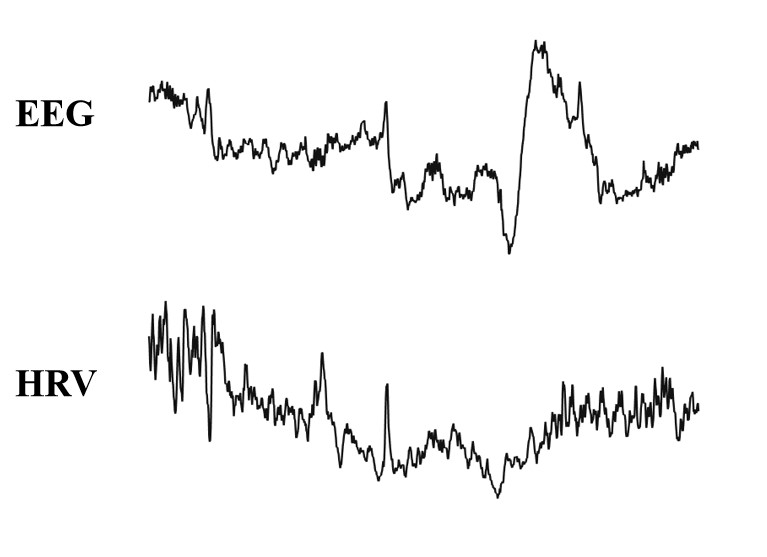
\includegraphics[height=5cm,width=8cm]{EEG-HRV.jpg}
%\caption{Examples of electrophysiological signals.}
%\label{signals01}
%\end{figure}


%These data are highly suited to machine learning algorithms, which automatically identify characteristics in electrophysiological signals and apply the information for depression-assisted diagnosis.
%Regarding the choice of machine learning algorithms, current research is still primarily based on traditional algorithms. At the same time, a few researchers have experimented with a subfield of machine learning - deep learning algorithms, which have made breakthroughs for related research. In what follows, this section will introduce both traditional machine learning and deep learning in the diagnosis of depression, respectively.




%In recent years, electrophysiological signals have been heavily researched to aid the diagnosis of depression, mainly including electroencephalography, electrocardiography, electrodermal, gastric, ophthalmic\cite{li2016classification}, and body temperature. Among them, EEG signals are one of the most promising. Because EEG is the most direct and objective representation of the neural activity of the human brain, it is closely linked to the brain's activity and emotional state, and can reflect the body's emotional changes in a timely manner.
%Based on these advantages of EEG, many researchers have investigated the detection of EEG signals in depression and have also tried many temporal sequence features and different machine learning classification models, including logistic regression classifiers, support vector machines, etc., achieving stage results. Further, with the development of deep learning, various deep learning network models have been applied to it, making breakthroughs for related research.
%In what follows, this section will look at both traditional machine learning in depression recognition and deep learning in depression recognition.

\subsection{EEG}


EEG is the most direct and objective representation of the neurological activity of the human brain. It is closely related to brain activity and emotional state, provides a timely reflection of the body's emotional changes, and provides a high temporal resolution for assessing brain dynamics. So the EEG is one of the most promising signals that can be employed to help with depression diagnosis.
%Therefore, among the physiological signals that can be used to assist in the diagnosis of depression, the EEG is one of the most promising.
Current research about EEG-based depression recognition is still primarily based on traditional machine learning algorithms. Meanwhile, a few researchers have experimented with a subfield of machine learning-deep learning algorithms, which have made breakthroughs for related research.


\subsubsection{EEG depression recognition based on traditional machine learning}

\begin{figure}
\centering
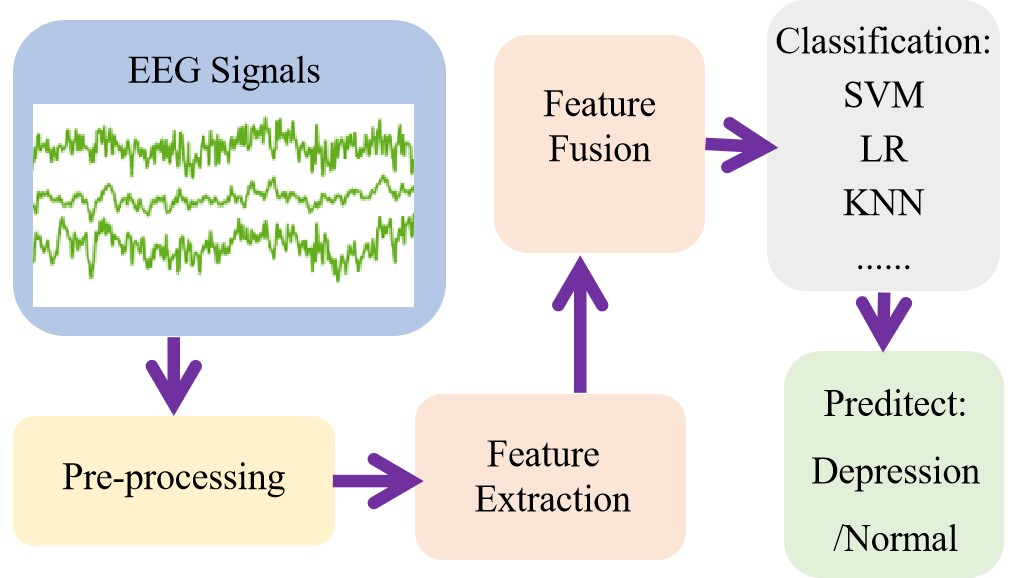
\includegraphics[width=1\linewidth]{eeg_tradition.jpg}
\caption{Flow diagram of EEG depression recognition using traditional machine learning.}
\label{eeg_traditional}
\end{figure}

The main process of EEG depression identification using traditional machine learning is shown in Fig~\ref{eeg_traditional}.
There are two key points to emphasize: feature extraction and classifiers.
According to the characteristics of EEG signals, feature extraction can be roughly  further summarized into two categories: linear and non-linear.
However, brain activity is inherently non-linear, and the EEG signal is non-stationary \cite{walleczek2006self,Scott2006encyclopedia,klonowski2006application}, which lead to limitations in the linear approach to assessing the dynamics of depressive EEG.
In contrast, the non-linear approach demonstrates a relatively clear advantage.
The non-linear dynamics theory suggests that a self-organizing, low-dimensional, deterministic system can generate complicated and non-periodic behavior that is inherent to the system rather than generated from external sources.
For such non-linear systems, numerous parameters have been discovered, including the correlation dimension \cite{akar2015nonlinear}, the Lyapunov exponent\cite{ortiz2021futility,kustubayeva2021lyapunov,chopra2022using}, and entropy \cite{zhao2019cardiorespiratory,cukic2018eeg,zhao2021frontal}.
The correlation dimension describes the system's complexity;
the largest Lyapunov exponent reflects the pace of uncertainty growth and is sensitive to the system's beginning value; and the entropy depicts the level of order in the system.
Researchers also employ a combination of multiple non-linear indictors because they can each reflect the distinctive properties of EEG from a different angle, exposing information that may not be picked up by other approaches.
For example, Acharya et al.\cite{acharya2015novel} presented a novel method for automated EEG-based diagnosis of depression using nonlinear methods: fractal dimension, largest Lyapunov exponent, sample entropy, detrended fluctuation analysis, Hurst's exponent, higher order spectra, and recurrence quantification analysis. The rational combination of the nonlinear features is used to diagnose depression.

%A novel depression diagnosis index is presented through judicious combination of the nonlinear features.

%
It was determined that depression had an effect on patients' EEG activity by comparing the distribution of linear and non-linear indicators between depressed patients and healthy controls.
Based on this, the researchers chose a few markers with strong discriminatory power to build a series of features for depression identification.
They then created a depression identification model based on different classifiers to achieve initial detection and diagnosis of depression.
Although the indicators utilized vary, the popular classifiers are usually the same, such as k-Nearest Neighbor (KNN), linear discriminant analysis, linear regression (LR), support vector machines (SVM), decision trees, Bayesian classifiers, random forests and probabilistic neural networks.
Hosseinifard et al. \cite{hosseinifard2013classifying} used associative dimensional features as input to a linear regression classifier and obtained 90\% recognition accuracy.
Ahmadlou et al.\cite{ahmadlou2012fractality} fed fractal dimensional features of depressed patients into an augmented probabilistic neural network and obtained an accuracy of 91.3\%.
Cukic et al. \cite{cukic2018eeg} obtained an accuracy of 90.24\%-97.56\% by feeding Higuchi fractal dimension and sample entropy into seven classifiers.


%As stated above, researchers use different physiological signals and features in physiological signal-based depression identification, which leads to slightly different outcomes.
%However, the the common classifiers are all consistent, including SVM, k-Nearest Neighbor (KNN), Logistic Regression (LR), and Random Forest (RF).

\subsubsection{EEG depression recognition based on Deep learning}
%\subsection{Application of deep learning in depression recognition}
%Applications of deep learning in depression diagnosis with the assistance of physiological signals have increased in recent times.
%All adopted models can be categorized into three main groups, namely Convolutional Neural Network (CNN)-Based models, Long-short Term Memory (LSTM) models, a hybrid neural network.
In recent years, deep learning has been utilized more and more to detect depression with the help of EEG.
All adopted models in these studies can be categorized into three main groups, namely Convolutional Neural Network (CNN) models\cite{wan2020hybrideegnet}, Long-short Term Memory (LSTM) models, and hybrid neural networks\cite{saeedi2021major,qayyum2020hybrid,thoduparambil2020eeg}. And their detailed flow is shown in Fig~\ref{eeg_cnn}.

\begin{figure}
\centering
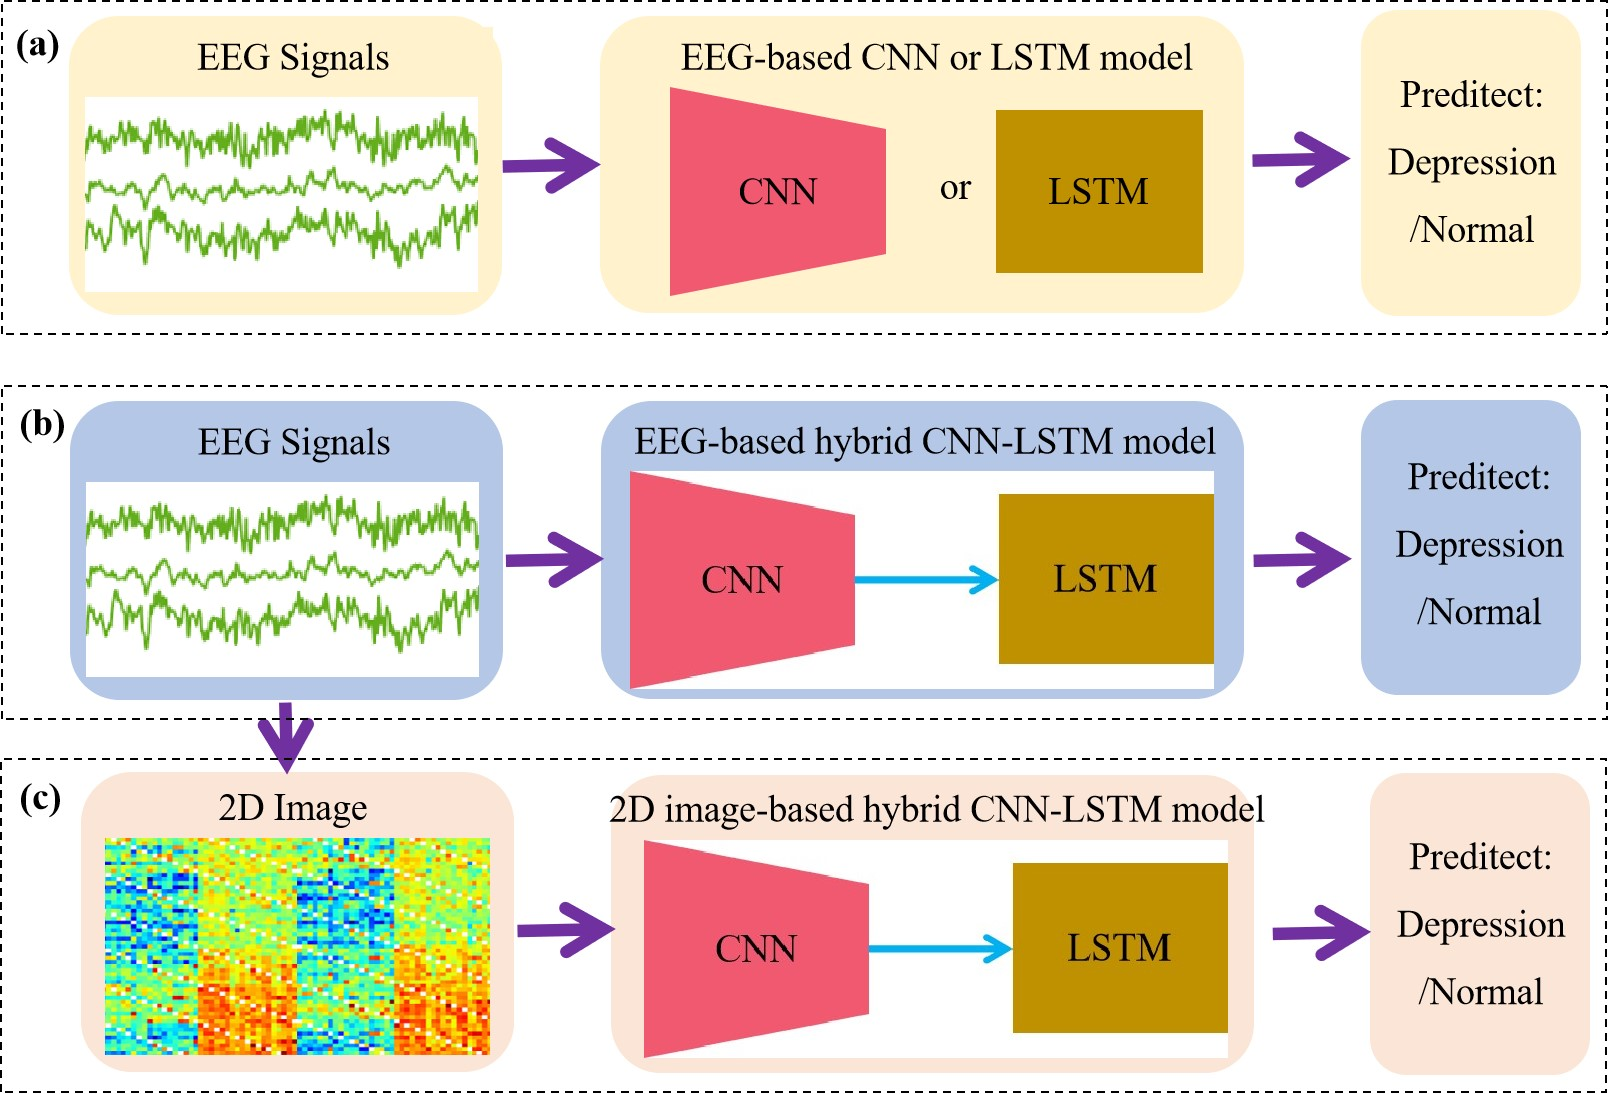
\includegraphics[width=1\linewidth]{eeg_cnn.jpg}
\caption{Flow diagram of EEG depression recognition based on deep learning. (a) Raw signal-based deep feature extraction and classification using CNN or LSTM; (b) raw signal-based deep feature extraction and classification using hybrid neural networks; (c) 2D image-based deep feature extraction and classification using hybrid neural networks. }
\label{eeg_cnn}
\end{figure}

In specific, %CNN could capture spatial properties of features and has the ability of parallel computing.
the CNN-based model can automatically and adaptively extract useful information directly from the input data instead of manually selecting features.
%Additionally, it has two significant groups of data input formats: time series and feature images.
Acharya et al.\cite{acharya2018automated} presented the first application of the deep neural network concept and CNN for diagnosis of depression.
The model's inputs were the EEG signals from the left and right hemispheres of the brain, respectively.
5 convolutional layers were responsible for providing important feature
obtained from the input EEG signals to train the algorithm, 5 pooling layers were accountable for reducing of the feature map's size, and 3 fully-connected layers established connection between neurons of a layer with the next one. Finally, results produced by the last fully-connected layer was applied to a soft-max function to detect depressive cases.
Similarly, Li et al.~\cite{li2019eeg} analyzed different aspects of EEG (spectral, spatial, and
temporal information) for the diagnosis of of mild depression. Results showed
that spectral information of EEG signals play major role whereas temporal information showed significant improvement in diagnostic performance. The uitlized the pre-trained ConvNet architectures on EEG-based mental load classification task and achieved accuracy of 85.62\% for recognition of mild depression and normal controls.
%Kang et al. \cite{kang2020deep} introduced a novel methodology of feature extraction to detect depression, which was exploiting asymmetry feature of EEG signals and converting it into 2D images.
%The produced image used as input of a CNN model which had constructed from three two-dimensional
%convolution layers with the ReLU as activation function, three two-dimensional max-pooling layers, one flatten and one dropout layer, and two fully connected layers.


%As a model capable of remembering long-term dependent information, LSTM can read and modify the long-term dependent information of a temporal sequence arbitrarily when processing temporal signals like EEG.
The benefit of the LSTM when processing temporal signals such as EEG is that it has the ability to read and modify the long-term dependent information of a temporal sequence at will\cite{alhagry2017emotion,wang2018lstm}.
Only a little portion of LSTM research, nevertheless, have focused on detecting depression through physiological signals.
Kumar et al. \cite{kumar2019prediction} researched depression prediction by the LSTM
model and the help of feature extraction.
To generate input data, time-domain analysis with moving window segmentation was
employed to extract the statistical mean feature. LSTM block comprised of one LSTM layer with ten hidden neurons, a dropout layer of 0.1, and a dense layer. They also compared the introduced method with two other models that were CNN-LSTM and ConvLSTM. Among them, LSTM had the best performance over those structures since it owned the smallest RMSE values (Root mean square error) as model evaluator rather than them.

The majority of the hybrid neural network are combined models of both CNN and LSTM blocks.
Additionally, it has two significant groups of data input formats: time series and feature images.
Concretely, Thoduparambil et al.\cite{thoduparambil2020eeg} designed a deep model in which an integration of CNN and LSTM is implemented for the detection of depression. Three CNN layers and three MaxPooling1D layers formed the first section of the model which exploited to extract features. The second unit
included two LSTM layers whose duty was to generate the feature maps by discovering different patterns in EEG signals and then retain the sequence of these learning.
Similarly, Sharma et al. \cite{sharma2021dephnn} also proposed a new hybrid neural network called DepHNN. CNN and LSTM are two deep learning algorithms used to capture the temporal dependencies in the time-series EEG input signals and to process the sequence learning, respectively.
Besides, Saeedi et al.~\cite{saeedi2021major} used brain effective connectivity method to convert 1D EEG signal into 2D image. Then, they developed a classifier using state of the art deep learning methods (CNN-LSTM) as a novel approach for automated diagnosis of the depression patients from EEG signals.
%The effectiveness of the proposed approach is tested on dataset recorded of from 33 MDD patients and 30 normal participants.
Finally, their experiments showed that the spatial and temporal characteristics of the EEG
signals are captured by 1DCNN-LSTM. Relying on the results, deep learning model is also capable
of effectively analyzing the brain connectivity.


%Besides, Kang et al. \cite{kang2020deep} introduced a novel methodology of feature extraction to detect depression, which was exploiting asymmetry feature of EEG signals and converting it into 2D images.
%%The produced image used as input of a CNN model which had constructed from three two-dimensional
%%convolution layers with the ReLU as activation function, three two-dimensional max-pooling layers, one flatten and one dropout layer, and two fully connected layers.




\subsubsection{Performance Comparison}

We evaluate the depression recognition method based on EEG.
The performance comparisons based on  traditional machine learning and deep learning are summarized in Table~\ref{tab_eeg}.
We would like to note that, we cannot comprehensively compare all studies because the dataset utilized vary, but by comparing the work from the same researchers, we can draw the following conclusion:

(1) Single-channel EEG analysis, employing the combination of measures, can provide the accuracy for discrimination of depression not lower than reported in other studies where multichannel EEG signals were analysed\cite{bachmann2018methods}.

(2)
The nonlinear analysis of EEG can be a useful method for discriminating depressed patients and normal subjects.
According to \cite{hosseinifard2013classifying}, the accuracy of three classifiers are
higher for all nonlinear features as the input in compare to power bands features.
Brain system is best-characterized non-linear dynamical process.
The nonlinearity of brain limits the ability of linear analysis to provide full description of underlying dynamics.

(3)
In contrast, the novelty of the deep learning model is that it does not require the employment of feature extraction, selection, and reduction. The model has the ability to self-learn and pick up distinctive features during training without a separate feature extraction or feature selection step.
Acharya\cite{acharya2018automated} presented the first application of the deep neural network concept for diagnosis of depression.
Even though the accuracy is not as great as the previous one\cite{acharya2015novel}, deep learning technology development is anticipated to lead to new discoveries.

\begin{table*}[!htbp]\Large
\caption{ Overview of machine learning based methods for Depression
Assessment from EEG.}
\label{tab_eeg}
\renewcommand\arraystretch{1.5}
%\resizebox{\linewidth}{!}{
\resizebox{0.9999\linewidth}{!}{%
\begin{threeparttable}
\begin{tabular}{c|cccccc}
\toprule
\textbf{Methods} & \textbf{Paper} & \textbf{Dataset} & \textbf{Feature} & \textbf{Classification} & \textbf{Metrics}           & \textbf{Value} \\ \midrule
& &  & FD, LLX, & & & \\
& &  & Hurst,HOS, & & & \\
& &  & SampEn, DFA &  &  & \\
& \multirow{-4}{*}{Acharya\cite{acharya2015novel}}  & \multirow{-4}{*}{15D+15C} & and RQA                                                                     & \multirow{-4}{*}{SVM} & \multirow{-4}{*}{Accuracy} & \multirow{-4}{*}{98.00} \\ \cline{2-7}
& & & SAI, APV and RGP & &  & Single-channel:92.00 \\
& \multirow{-2}{*}{Bachmnn\cite{bachmann2018methods}} & \multirow{-2}{*}{13D+13C}  & HFD, DFA and Lempel-Ziv & \multirow{-2}{*}{LR} & \multirow{-2}{*}{Accuracy} & Multil-channel:90.00  \\ \cline{2-7}
& &  & Power & KNN &  & Linear/Nonlinear:73.3/80   \\
& & & DFA, HFD, CD  & LDA& & Linear/Nonlinear:76.6/86.6 \\
\textbf{EEG} & \multirow{-3}{*}{Hosseinifard\cite{hosseinifard2013classifying}} & \multirow{-3}{*}{45D+45C} & and lyapunov exponent & LR& \multirow{-3}{*}{Accuracy} & Linear/Nonlinear:76.6/90   \\ \cline{2-7}
\textbf{depression} & & && Multilayer perceptron &  & 95.12  \\
\textbf{recognition} & & & & LR &  & 97.56  \\
\textbf{based on} & &  & & SVM with linear kernel &  & 95.12  \\
\textbf{traditional} &  & &  & SVM with polynomial & & 95.12   \\
\textbf{machine}&  & &  & Decision tree  &  & 95.12  \\
\textbf{learning} &  & & & Random forest && 92.68  \\
& \multirow{-7}{*}{Cukic\cite{cukic2018eeg}}  & \multirow{-7}{*}{23D+20C} & \multirow{-7}{*}{HFD,SampEn}                                                              & Naive Bayes& \multirow{-7}{*}{Accuracy} & 92.68 \\ \cline{2-7}
& Ahmadlou\cite{ahmadlou2012fractality} & 12D+12C & FD & EPNN & Accuracy & 91.30 \\ \cline{2-7}
& Faust\cite{faust2014depression} & 30D+30C& ApEn, SampEn, REN and Ph & PNN& Accuracy & 99.7  \\ \cline{2-7}
& Liao\cite{liao2017major} & 12D+12C  & KEFBCS& SVM & Accuracy & 80.00 \\ \midrule
& Wan\cite{wan2020hybrideegnet}  & 23D+12C  & Raw signals  & HybridEEGNet& Accuracy & 79.08 \\ \cline{2-7}
& Saeedi\cite{saeedi2021major} & 34D+30C & Effective connectivity & 1DCNN-LSTM & Accuracy & 99.24 \\ \cline{2-7}
& Quayyam\cite{qayyum2020hybrid}  & & Raw signals & 1DCNN-GRU-RF & F1-score & 99.94 \\ \cline{2-7}
\textbf{EEG} & &  &  & & & Left hemisphere:98.84 \\
\textbf{depression}& \multirow{-2}{*}{Thoduparambil\cite{thoduparambil2020eeg}} & \multirow{-2}{*}{ } & \multirow{-2}{*}{Raw signals} & \multirow{-2}{*}{CNN-LSTM}  & \multirow{-2}{*}{Accuracy} & Right hemisphere:99.07     \\ \cline{2-7}
\textbf{recognition} & & &  &  & & Left hemisphere:93.5       \\
\textbf{based on} & \multirow{-2}{*}{Acharya\cite{acharya2018automated}} & \multirow{-2}{*}{15D+15C} & \multirow{-2}{*}{Raw signals} & \multirow{-2}{*}{CNN} & \multirow{-2}{*}{Accuracy} & Right hemisphere:96.0      \\ \cline{2-7}
\textbf{deep} & Kang\cite{kang2020deep} & 34D+30C  & Asymmetry matrix image & CNN  & Accuracy & 98.85 \\  \cline{2-7}
\textbf{learning}& Kumar\cite{kumar2019prediction} & 30D & time domain feature& LSTM  & RMSE  & 0.005 \\ \cline{2-7}
& Sharma\cite{sharma2021dephnn} & 21D+24C & Raw signals & DepHNN & Accuracy & 99.1  \\ \cline{2-7}
& Li\cite{li2019eeg} & 24D+24C& spectral, spatial, and temporal information & ConvNet & Accuracy & 85.62  \\ \cline{2-7}
& &  &  &  &  & Left hemisphere:99.12      \\
& \multirow{-2}{*}{Ay\cite{ay2019automated}} & \multirow{-2}{*}{15D+15C} & \multirow{-2}{*}{Raw signals}                                                                              & \multirow{-2}{*}{CNN-LSTM}  & \multirow{-2}{*}{Accuracy} & Right hemisphere:97.66\\ \bottomrule
\end{tabular}
      \begin{tablenotes} %���Ӵ˴�
		\item Largest Lyapunov exponent: LLX; Higher order spectra: HOS; Recurrence quantification analysis: RQA;
              Spectral asymmetry index: SAI;
        \item Alpha power variability: APV; Relative gamma power: RGP; Detrended fluctuation analysis: DFA; Linear discriminant analysis: LDA; Sample Entropy: SampEn; % ���Ӵ˴�
        Fractal Dimension: FD; Enhanced probabilistic neural network: EPNN;
        approximate entropy: ApEn; Renyi entropy: REN; Bispectral phase entropy: Ph; Kernel eigen-filter-bank common spatial pattern: KEFBCS.
     \end{tablenotes} %���Ӵ˴�
\end{threeparttable}}
\end{table*}



\subsection{ECG}



Depression is associated with the autonomic nervous system (ANS) dysfunction \cite{jandackova2016heart}.
Heart rate variability (HRV), levels of variability of the heart beat-to-beat interval over time, has been known to provide an index of ANS functioning including the sympathetic and parasympathetic system \cite{heart1996standards}.
Many studies have demonstrated automated detection using HRV in patients with major depression using machine learning methods.

%Depression patients show reduced parasympathetic modulation.
%Because heart rate variability (HRV) is governed by the dynamic equilibrium between sympathetic and parasympathetic nerves, it can be used to evaluate ANS modulation.
%Heart rate variability is controlled by the dynamic balance of sympathetic and parasympathetic nerves, so the state of autonomic activity can be assessed by analyzing the sequence of heart rate variability.

\subsubsection{HRV depression recognition based on traditional machine learning}

In terms of classic approaches, the fundamental steps of EEG-based depression identification and HRV-based depression identification are similar.
Particularly, the signal's multidimensional features are first extrated, then a classification  model is built, and finally this model is applied to diagnosis depression.
The most commonly used features to quantify HRV signals are time-domain and
frequency-domain features.
%The most commonly used features to quantify HRV signals are time-domain and
%frequency-domain features, which are used in most studies to study HRV in patients with depression.
Time-domain HRV features can be calculated directly from the time series of R-peak to R-peak interval (RRI)\cite{sgoifo2015autonomic}.
The mean and standard deviation of RRIs (SDNN)\cite{shaffer2017overview}, the root mean square of successive RR interval differences (RMSSD), and the percentage of successive RRIs differing by more than 50ms (PNN50) are all commonly used time domain features\cite{schneider2017validity}.
Whereas the mean of RRIs measures the intensity of HRV \cite{colombo2015clinical}, the SDNN measures overall HRV and reflects both sympathetic and parasympathetic activity in the autonomic nervous system\cite{byun2019detection}, and the RMSSD and PNN50 are more sensitive to parasympathetic modulation.



Frequency-domain provides an assessment of vagal modulation of the RRI, extracted from the ECG.
It is mostly commonly acquired by fast Fourier transformation (FFT).
The RRI can be separated into three components depending on the frequency band: very low frequency (VLF, 0.003-0.04 Hz), low frequency (LF, 0.04-0.15 Hz), and high frequency (HF, 0.15-0.4 Hz) band \cite{kidwell2018heart}. According to previous studies, HF is primarily affected by parasympathetic activities while LF is influenced by both sympathetic and parasympathetic activity.
The ratio of LF to HF indicates that sympathetic activity predominates as compared to parasympathetic activity\cite{billman2013lf}.




The typical HRV markers mentioned above are frequently used to detect depression as well.
Kemp~\cite{kemp2012depression} summarized the achievements of numerous researchers and discovered that depressive individuals had much lower SDNN and RMSDD values in the time domain, HF values in the frequency domain, and HF/LF values in the frequency domain than healthy controls.
The differences in HRV between individuals with severe depression and healthy controls have been further investigated in numerous subsequent research.
Additionally to these markers, it was discovered that compared to healthy participants, depressive patients exhibited considerably lower PNN50 in the temporal domain and greater LF in the frequency domain~\cite{shinba2014altered}.

%As heart rate fluctuation is a complex behavior originating from nonlinear regulatory processes, adaptation of nonlinear dynamics and information theory for HRV analysis has been suggested.
Although HRV has been analyzed traditionally using linear methods, such as time-domain and frequency-domain analyses, growing evidence has demonstrated that linear HRV measures may not correctly represent the complex dynamics of heartbeat regulation modulated by the ANS~\cite{goldberger2002fractal}and that linear HRV features show a relatively higher inter-subject variability than nonlinear HRV indices, suggesting the importance of nonlinear HRV analysis.
Schulz et al.~\cite{schulz2010altered} have shown that nonlinear HRV indices allow more reliable discrimination of major depressive disorder (MDD) patients from controls than linear HRV features, as the latter exhibit high inter-subject variability.
In particular, the non-linear features used for EEG: fractal dimension, Lyapunov's index, entropy, etc., also apply to HRV.
Greco et al. \cite{greco2018assessment} found that non-linear indicators such as fractal dimension, sample entropy and recursive graph analysis demonstrated significantly higher heart rate variability even in subclinical depression compared to healthy controls.
Daniel et al. \cite{vigo2004relation}found that depressed patients over 60 years of age had significantly lower sample entropy values compared to healthy controls.



In order to recognize depression using HRV, a variety of classifiers can be used.
Kang et al. \cite{kuang2017depression} used the bayesian network to recognition depressed patients from a healthy people, the recognition results demonstrate the significant association between depression and HRV.
Byun et al.~\cite{byun2019detection} demonstrated the HRV-based diagnosis of MDD using SVM classifier. Monitoring the changes in linear and nonlinear HRV features for various autonomic nervous system states can facilitate the more objective identification of MDD patients.


\subsubsection{HRV depression recognition based on deep learning}
Although traditional machine learning techniques perform well, they nevertheless have several shortcomings, which are dependence on feature extraction and feature selection to a large extent.
It indicates that the procedure consequently becomes both time and computationally-intensive.
Unlike traditional machine learning, deep learning can automatically learn features from input data, therefore researchers are trying to use it to diagnose depression.
Noor et al.~\cite{noor2021predicting} presented a model that used Recurrent Neural Network (RNN)and LSTM to predict the risk of depression based on HRV.
zang et al.~\cite{zang2022end} proposed a CNN network containing 2 convolutional layers, 2 max pooling layers and 1 fully connected layer to diagnose depression, and the results showed that the network achieved high classification performance.
In conclusion, the end-to-end deep learning approach can identify depression from HRV signals, and possess high diagnostic performance.

%Although traditional approaches perform well in terms of classification, they also have significant flaws.
%For instance, HRV sequences are typically reflected in the ECG signal by variations in the RR interval.
%Nevertheless, various QRS wave detection techniques provide varying R points, which may have an impact on the classification outcomes of succeeding classifiers.
%Additionally, feature extraction and feature selection play a significant role in machine learning.
%This method requires a lot of computation in addition to time.
%Instead of requiring human feature extraction and feature selection, deep learning-based algorithms can learn features from the input signal on their own.
%For these reasons, researchers have tried to detect depression directly from ECG data using deep learning techniques.



\subsubsection{Performance Comparison}
%Table \ref{tab_ecg} summarizes the results of the experiments on the detection of depression based on HRV, including the source and name of the method, the data set used, the evaluation criteria of the experimental results.

Previous studies in which ECG/HRV features were used to discriminate depression patients have yielded promising results obtained via various machine learning methods, which are summarized in Table~\ref{tab_ecg}.
In these studies, Kuang et al.~\cite{kuang2017depression} achieved an accuracy of 86\% through selected HRV features, but only female subjects participated in this study; Zhang et al.~\cite{zhang2011new} used relatively small sample sizes. Traditional studies have used HRV features to discriminate patients with depression, and HRV is usually expressed from the RR interval collected from ECG data. It is inevitable that the QRS wave algorithm will be utilized to locate R-peak. The R-peak positioned by different QRS wave algorithms also has biases.
On the contrary, the deep learning method directly takes the ECG signal as input without extracting the HRV sequence.
In addition, traditional studies used simple classifiers to train features manually extracted from HRV sequences.
The performance of this type of classifier mainly depends on the feature selection process, which is laborious and time-consuming.
The deep model can overcome the shortcomings of manual feature extraction and selection.


%This research used data from 37 depressed patients and 37 normal controls. Small samples limit the use of other deep neural network models.


%Some previous studies [11, 12, 38] focused on classifying patients with major depressive disorder and healthy people, thus ignoring the identification of mild and moderate patients.


\begin{table*}[!htbp]\Large
\caption{ Overview of machine learning based methods for Depression
Assessment from HRV.}
\label{tab_ecg}
\renewcommand\arraystretch{1.5}
%\resizebox{\linewidth}{!}{
\resizebox{0.9999\linewidth}{!}{%
\begin{threeparttable}
\begin{tabular}{c|cccccc}
\toprule
\textbf{Methods} & \textbf{Paper} & \textbf{Dataset}  & \textbf{Feature} & \textbf{Classification} & \textbf{Metrics}           & \textbf{Value}  \\ \midrule
   & Zhang\cite{zhang2011new} & 10D+10C & VLF,LF,HF,LF/HF,SDNN,RMSSD & Neuro-fuzzy network & Accuracy& 95.00 \\
&  & & RRI,SDNN,RMSSD,PNN50,TRI,TINN, & & &  \\
& & & VLF,LF,HF,LF/HF,Tot & \multirow{-2}{*}{SVM} & \multirow{-2}{*}{Accuracy} & \multirow{-2}{*}{74.4} \\
HRV depression recognition & &  & ApEn,SampEn,DFA,CD, & &  & \\
based on traditional  & \multirow{-4}{*}{Byuna\cite{byun2019detection}}    & \multirow{-4}{*}{31D+41C} & SD1,SD2 & \multirow{-2}{*}{Statistical filter} & \multirow{-2}{*}{Accuracy} & \multirow{-2}{*}{73.1} \\
machine learning & &  & HR,SDNN,PNN50, &  &  &  \\
& & & LF/HF,peakLF,peakHF,  &  &   &      \\
& \multirow{-3}{*}{Roh\cite{roh2014wearable}} & \multirow{-3}{*}{23D}  & LLE,SampEn,ApEn & \multirow{-3}{*}{SVM}                & \multirow{-3}{*}{Accuracy} & \multirow{-3}{*}{71}   \\
& Matsui\cite{matsui2016impaired}  & 13D+28C  & LF,HF  & LDA  & Accuracy  & 88  \\
& Sun\cite{sun2016objective} & 44D+47C & LF,HF,LF/HF  & Logistic regression & Accuracy & 79  \\
& & & SDNN,RMSSD,SDSD,PNN50,MEAN &  & &  \\
& & & VLF,LF,HF,  & &  &   \\
& \multirow{-3}{*}{Kuang\cite{kuang2017depression}} & \multirow{-3}{*}{38D+38C} & SampEn,DFA & \multirow{-3}{*}{Bayesian networks}  & \multirow{-3}{*}{Accuracy} & \multirow{-3}{*}{86}   \\  \midrule
HRV depression recognition & Noor\cite{noor2021predicting} & 5000D& Raw signals  & RNN    & Accuracy & 97.24 \\
recognition based on & zang\cite{zang2022end}   & 37D+37C & Raw signals& CNN & Accuracy & 93.96 \\
deep learning& Mohanraj\cite{mohanraj2022deep}  & 15D+15C & Raw signals & DesNN  & Accuracy & 90 \\ \bottomrule
\end{tabular}
      \begin{tablenotes} %���Ӵ˴�
		\item Standard deviation of the successive difference of RR intervals: SDSD; Mean value of RR intervals: MEAN;
      	Integral of the histogram of the RR interval divided by its height: TRI; Baseline width of the RR interval histogram:TINN; Total power: Tot; Standard deviation of the Poincar�� plot perpendicular to (SD1) and along (SD2) the line of identity: SD1, SD2.
     \end{tablenotes} %���Ӵ˴�
\end{threeparttable}}
\end{table*}



\subsection{EM}

%Eye Movements (EM) are the numerous types of eye movements that the human eye displays after receiving external visual information.
EM refers to the voluntary and involuntary movements of the eyes that assist with obtaining, fixating and following visual stimuli.
EM information, which includes object gaze, gaze duration, gaze displacement, and pupil size, provides a clear indicator of the information-processing mechanisms at work in the brain and can be used to characterize how emotions are perceived by individuals.
Therefore, EM is often used as the primary measure of emotion and mood.


The researchers observed, measured, and recorded the experimental participants' EM characteristics through a variety of task paradigms, which can be categorised into saccade, gaze, memory and free-viewing tasks.
EM measures used on saccade tasks include saccade gain, saccade error rate and task mistake rate. These metrics are related to cognitive ability.
Sweeney et al. \cite{sweeney1998prefrontal} found that depressed patients demonstrated increased rates of response suppression errors on an antisaccade task.
The gaze-type task examines the subject's capacity to suppress eye-hopping and is linked to brain function in the dorsolateral prefrontal cortex (DLPFC).
In the memory task, subjects must first fixate on a central point while being prohibited from moving their gaze towards the goal, which appears in the peripheral vision.
After the peripheral target disappears they are asked to eye skip towards the target area from memory, while eye skip latencies are recorded and error rates are used to assess damage to the basal ganglia and frontal regions.
Studies have revealed that depressed patients have higher error rates for eye skipping than normal controls.
A free-viewing task, which measures attentional bias, is usually achieved by viewing pictures of emotional faces.
According to Duque et al.\cite{duque2015double}, major depressive patients had a negative affective bias, or a longer duration of first look and total gaze on negative emotional faces than normal controls, which was positively connected with the severity of depressed symptoms.







New developments in the diagnosis of depression using eye-movement measurements have been made possible by the development of machine learning.
li et al.\cite{li2020method} used statistical methods (FDR correction and t-test) and PCA to screen behavioral features as well as eye-movement features, and finally achieved a 91\% depression recognition rate using a kernel-limit learning machine.
Pan et al.\cite{pan2019depression} extracted reaction time features reflecting subjects' attentional bias as well as eye-movement features and used SVM to achieve 86\% classification accuracy for both depressed and normal categories.
Lu et al. \cite{lu2020depression} used a particle swarm algorithm to optimise the regularisation and kernel parameters in an extreme learning machine and used eye-movement data to classify both normal and depressed people, achieving a classification accuracy of 88.55\%.








% Please add the following required packages to your document preamble:
% \usepackage{multirow}
% \usepackage[table,xcdraw]{xcolor}
% If you use beamer only pass "xcolor=table" option, i.e. \documentclass[xcolor=table]{beamer}
% Please add the following required packages to your document preamble:
% \usepackage{multirow}
% \usepackage[table,xcdraw]{xcolor}
% If you use beamer only pass "xcolor=table" option, i.e. \documentclass[xcolor=table]{beamer}





\ifx\allfiles\undefined
% !TEX root = tnnls_relation_gait.tex

% if have a single appendix:
%\appendix[Proof of the Zonklar Equations]
% or
%\appendix  % for no appendix heading
% do not use \section anymore after \appendix, only \section*
% is possibly needed

% use appendices with more than one appendix
% then use \section to start each appendix
% you must declare a \section before using any
% \subsection or using \label (\appendices by itself
% starts a section numbered zero.)
%

%\appendices
%\section{Proof of the First Zonklar Equation}
%Appendix one text goes here.
%
%% you can choose not to have a title for an appendix
%% if you want by leaving the argument blank
%\section{}
%Appendix two text goes here.

% use section* for acknowledgment
% \section*{Acknowledgment}
% The authors would like to thank Prof. Dongbin Zhao for his support to this work.

% Can use something like this to put references on a page
% by themselves when using endfloat and the captionsoff option.
\ifCLASSOPTIONcaptionsoff
  \newpage
\fi

% trigger a \newpage just before the given reference
% number - used to balance the columns on the last page
% adjust value as needed - may need to be readjusted if
% the document is modified later
%\IEEEtriggeratref{8}
% The "triggered" command can be changed if desired:
%\IEEEtriggercmd{\enlargethispage{-5in}}

% references section

% can use a bibliography generated by BibTeX as a .bbl file
% BibTeX documentation can be easily obtained at:
% http://mirror.ctan.org/biblio/bibtex/contrib/doc/
% The IEEEtran BibTeX style support page is at:
% http://www.michaelshell.org/tex/ieeetran/bibtex/
\bibliographystyle{IEEEtran}
% argument is your BibTeX string definitions and bibliography database(s)
\bibliography{IEEEabrv,tnnls_relation_gait}
%
% <OR> manually copy in the resultant .bbl file
% set second argument of \begin to the number of references
% (used to reserve space for the reference number labels box)
%\begin{thebibliography}{1}
%\bibitem{IEEEhowto:kopka}
%H.~Kopka and P.~W. Daly, \emph{A Guide to \LaTeX}, 3rd~ed.\hskip 1em plus
%  0.5em minus 0.4em\relax Harlow, England: Addison-Wesley, 1999.
%\end{thebibliography}

% biography section
%
% If you have an EPS/PDF photo (graphicx package needed) extra braces are
% needed around the contents of the optional argument to biography to prevent
% the LaTeX parser from getting confused when it sees the complicated
% \includegraphics command within an optional argument. (You could create
% your own custom macro containing the \includegraphics command to make things
% simpler here.)
%\begin{IEEEbiography}[{\includegraphics[width=1in,height=1.25in,clip,keepaspectratio]{mshell}}]{Michael Shell}
% or if you just want to reserve a space for a photo:

%\begin{IEEEbiography}{Michael Shell}
%Biography text here.
%\end{IEEEbiography}
%
%% if you will not have a photo at all:
%\begin{IEEEbiographynophoto}{John Doe}
%Biography text here.
%\end{IEEEbiographynophoto}

% insert where needed to balance the two columns on the last page with
% biographies
% \newpage

%\begin{IEEEbiographynophoto}{Jane Doe}
%Biography text here.
%\end{IEEEbiographynophoto}

%\begin{IEEEbiography}[{\includegraphics[width=1in,height=1.25in,clip,keepaspectratio]{photos/hsh.pdf}}]{Saihui Hou}
%% \begin{IEEEbiographynophoto}{Saihui Hou}
%	received the B.E. and Ph.D. degrees from University of Science and Technology of China in 2014 and 2019, respectively.
%    %
%    He is currently an Assistant Professor with School of Artificial Intelligence, Beijing Normal University.
%    %
%    His research interests include computer vision and machine learning.
%    %
%    He focuses on gait recognition which aims to identify different people according to the walking patterns.
%% \end{IEEEbiographynophoto}
%\end{IEEEbiography}
%
%\begin{IEEEbiography}[{\includegraphics[width=1in,height=1.25in,clip,keepaspectratio]{photos/lx.pdf}}]{Xu Liu}
%% \begin{IEEEbiographynophoto}{Xu Liu}
%	received the B.E. and Ph.D. degrees from University of Science and Technology of China in 2013 and 2018, respectively.
%    %
%    He is currently a Research Scientist with Watrix Technology Limited Co. Ltd.
%    %
%    His research interests include gait recognition, object detection and image segmentation.
%% \end{IEEEbiographynophoto}
%\end{IEEEbiography}
%
%\begin{IEEEbiography}[{\includegraphics[width=1in,height=1.25in,clip,keepaspectratio]{photos/ccs.pdf}}]{Chunshui Cao}
%% \begin{IEEEbiographynophoto}{Chunshui Cao}
%	received the B.E. and Ph.D. degrees from University of Science and Technology of China in 2013 and 2018, respectively.
%    %
%    During his Ph.D. study, he joined Center for Research on Intelligent Perception and Computing, National Laboratory of Pattern Recognition, Institute of Automation, Chinese Academy of Sciences.
%    %
%    From 2018 to 2020, he worked as a Postdoctoral Fellow with PBC School of Finance, Tsinghua University.
%    %
%    He is currently a Research Scientist with Watrix Technology Limited Co. Ltd.
%    %
%    His research interests include pattern recognition, computer vision and machine learning.
%% \end{IEEEbiographynophoto}
%\end{IEEEbiography}
%
%\begin{IEEEbiography}[{\includegraphics[width=1in,height=1.25in,clip,keepaspectratio]{photos/hyz.pdf}}]{Yongzhen Huang}
%% \begin{IEEEbiographynophoto}{Yongzhen Huang}
%	received the B.E. degree from Huazhong University of Science and Technology in 2006, and the Ph.D. degree from Institute of Automation, Chinese Academy of Sciences in 2011.
%    %
%    He is currently an Associate Professor with School of Artificial Intelligence, Beijing Normal University.
%    %
%    He has published one book and more than 80 papers at international journals and conferences such as TPAMI, IJCV, TIP, TSMCB, TMM, TCSVT, CVPR, ICCV, ECCV, NIPS, AAAI.
%    %
%    His research interests include pattern recognition, computer vision and machine learning.
%% \end{IEEEbiographynophoto}
%\end{IEEEbiography}


\end{document}

\fi
